%package list
\documentclass{article}
\usepackage[top=3cm, bottom=3cm, outer=3cm, inner=3cm]{geometry}
\usepackage{multicol}
\usepackage{graphicx}
\usepackage{url}
%\usepackage{cite}
\usepackage{hyperref}
\usepackage{array}
%\usepackage{multicol}
\newcolumntype{x}[1]{>{\centering\arraybackslash\hspace{0pt}}p{#1}}
\usepackage{natbib}
\usepackage{pdfpages}
\usepackage{multirow}
\usepackage[normalem]{ulem}
\useunder{\uline}{\ul}{}
\usepackage{svg}
\usepackage{xcolor}
\usepackage{listings}
\lstdefinestyle{ascii-tree}{
	literate={├}{|}1 {─}{--}1 {└}{+}1 
}
\lstset{basicstyle=\ttfamily,
	showstringspaces=false,
	commentstyle=\color{red},
	keywordstyle=\color{blue}
}
%\usepackage{booktabs}
\usepackage{caption}
\usepackage{subcaption}
\usepackage{float}
\usepackage{array}

\newcolumntype{M}[1]{>{\centering\arraybackslash}m{#1}}
\newcolumntype{N}{@{}m{0pt}@{}}


%%%%%%%%%%%%%%%%%%%%%%%%%%%%%%%%%%%%%%%%%%%%%%%%%%%%%%%%%%%%%%%%%%%%%%%%%%%%
%%%%%%%%%%%%%%%%%%%%%%%%%%%%%%%%%%%%%%%%%%%%%%%%%%%%%%%%%%%%%%%%%%%%%%%%%%%%
\newcommand{\itemEmail}{aalfonso@unsa.edu.pe}
\newcommand{\itemStudent}{Repositorio: proyecto}
\newcommand{\itemCourse}{PWEB 2}
\newcommand{\itemCourseCode}{20220596}
\newcommand{\itemSemester}{I}
\newcommand{\itemUniversity}{Universidad Nacional de San Agustín de Arequipa}
\newcommand{\itemFaculty}{Facultad de Ingeniería de Producción y Servicios}
\newcommand{\itemDepartment}{Departamento Académico de Ingeniería de Sistemas e Informática}
\newcommand{\itemSchool}{Escuela Profesional de Ingeniería de Sistemas}
\newcommand{\itemAcademic}{2023 - A}
\newcommand{\itemInput}{Del 29 Junio 2023}
\newcommand{\itemOutput}{Al 14 Julio 2023}
\newcommand{\itemPracticeNumber}{07}
\newcommand{\itemTheme}{Relaciones de uno a muchos, muchos a muchos y impresion de pdf y emails}
%%%%%%%%%%%%%%%%%%%%%%%%%%%%%%%%%%%%%%%%%%%%%%%%%%%%%%%%%%%%%%%%%%%%%%%%%%%%
%%%%%%%%%%%%%%%%%%%%%%%%%%%%%%%%%%%%%%%%%%%%%%%%%%%%%%%%%%%%%%%%%%%%%%%%%%%%

\usepackage[english,spanish]{babel}
\usepackage[utf8]{inputenc}
\AtBeginDocument{\selectlanguage{spanish}}
\renewcommand{\figurename}{Figura}
\renewcommand{\refname}{Referencias}
\renewcommand{\tablename}{Tabla} %esto no funciona cuando se usa babel
\AtBeginDocument{%
	\renewcommand\tablename{Tabla}
}

\usepackage{fancyhdr}
\pagestyle{fancy}
\fancyhf{}
\setlength{\headheight}{30pt}
\renewcommand{\headrulewidth}{1pt}
\renewcommand{\footrulewidth}{1pt}
\fancyhead[L]{\raisebox{-0.2\height}{
\includegraphics[width=3cm]{img/logo_episunsa.png}}}
\fancyhead[C]{\fontsize{7}{7}\selectfont	\itemUniversity \\ \itemFaculty \\ \itemDepartment \\ \itemSchool \\ \textbf{\itemCourse}}
\fancyhead[R]{\raisebox{-0.2\height}{
\includegraphics[width=1.2cm]{img/logo_abet}}}
\fancyfoot[L]{Estudiante Sebastian Alfonso Huacasi}
\fancyfoot[C]{\itemCourse}
\fancyfoot[R]{Página \thepage}

% para el codigo fuente
\usepackage{listings}
\usepackage{color, colortbl}
\definecolor{dkgreen}{rgb}{0,0.6,0}
\definecolor{gray}{rgb}{0.5,0.5,0.5}
\definecolor{mauve}{rgb}{0.58,0,0.82}
\definecolor{codebackground}{rgb}{0.95, 0.95, 0.92}
\definecolor{tablebackground}{rgb}{0.8, 0, 0}

\lstset{frame=tb,
	language=bash,
	aboveskip=3mm,
	belowskip=3mm,
	showstringspaces=false,
	columns=flexible,
	basicstyle={\small\ttfamily},
	numbers=none,
	numberstyle=\tiny\color{gray},
	keywordstyle=\color{blue},
	commentstyle=\color{dkgreen},
	stringstyle=\color{mauve},
	breaklines=true,
	breakatwhitespace=true,
	tabsize=3,
	backgroundcolor= \color{codebackground},
}

\begin{document}
	
	\vspace*{10px}

\begin{center}	
	\fontsize{17}{17} \textbf{ Informe de Laboratorio 07}
\end{center}
\centerline{\textbf{\Large Tema: Relaciones de uno a muchos, muchos a muchos y impresion de pdf y emails}}
%\vspace*{0.5cm}	

\begin{flushright}
	\begin{tabular}{|M{2.5cm}|N|}
		\hline 
		\rowcolor{tablebackground}
		\color{white} \textbf{Nota}  \\
		\hline 
		\\[30pt]
		\hline 			
	\end{tabular}
\end{flushright}	

\begin{table}[H]
	\begin{tabular}{|x{4.7cm}|x{4.8cm}|x{4.8cm}|}
		\hline 
		\rowcolor{tablebackground}
		\color{white} \textbf{Estudiantes} & \color{white}\textbf{Escuela}  & \color{white}\textbf{Asignatura}   \\
		\hline 
		{- Alejandro Sebastian Alfonso Huacasi \par aalfonso@unsa.edu.pe \par} & Escuela Profesional de Ingenieria de Sistemas & {Programación web 2 \par Semestre: A}     \\
		\hline 			
	\end{tabular}
\end{table}		

\begin{table}[H]
	\begin{tabular}{|x{4.7cm}|x{4.8cm}|x{4.8cm}|}
		\hline 
		\rowcolor{tablebackground}
		\color{white}\textbf{Laboratorio} & \color{white}\textbf{Tema}  & \color{white}\textbf{Duración}   \\
		\hline 
		07 & Relaciones de uno a muchos, muchos a muchos y impresion de pdf y emails & 04 horas   \\
		\hline 
	\end{tabular}
\end{table}

\begin{table}[H]
	\begin{tabular}{|x{4.7cm}|x{4.8cm}|x{4.8cm}|}
		\hline 
		\rowcolor{tablebackground}
		\color{white}\textbf{Semestre académico:} & \color{white}\textbf{Fecha de inicio}  & \color{white}\textbf{Fecha de entrega}   \\
		\hline 
		2023 - A & Del 29 Junio 2023 &  Al 14 Julio 2023  \\
		\hline 
	\end{tabular}
\end{table}
	
	TAREA
\begin{itemize}		
	\item Reproducir las actividades de los videos donde trabajamos:
	\item Relación de uno a muchos
        \item Relación muchos a muchos
        \item Impresión de pdfs 
        \item Envio de emails
\end{itemize}

		
	\section{Equipos, materiales y temas utilizados}
\begin{itemize}
	\item Sistema Operativo (GNU/Linux de preferencia).
	\item GNU Vim.
	\item Python 3
	\item Git.
	\item Cuenta en GitHub con el correo institucional.
        \item Entorno virtual
        \item Django 4
\end{itemize}
	
	\section{URL DE MI REPOSITORIO DE GIT HUB}
\begin{itemize}
	\item \url{https://github.com/Sebastianzzzin/proyecto.git}
\end{itemize}
	
	\section{Actividades con el repositorio GitHub}

\subsection{Creando e inicializando repositorio GitHub}
\begin{itemize}	
	\item Como ya tenemos nuestro repositorio GitHub y además esta clonado e inicializado en nuestra máquina local.
	\item Se realizaron los siguientes comandos en la computadora:
\end{itemize}	

\begin{lstlisting}[language=bash,caption={Creando carpeta de trabajo dentro de nuestro repositorio clonado en mi maquina local}][H]
	$ cd proyecto
   $ mkdir lab07
\end{lstlisting}
\begin{lstlisting}[language=bash,caption={Dirijíéndonos a la carpeta de trabajo}][H]
	$ cd lab07
\end{lstlisting}	
\begin{lstlisting}[language=bash,caption={Creando carpetas que contendrán el proyecto e imagenes}][H]
	$ cd lab07
   $ mkdir emailexample
   $ mkdir model_examples
   $ mkdir pdfs_examples
\end{lstlisting}

\subsection{Commits}
\begin{itemize}	
	\item A continucación se mostraran capturas de los commits, primero de la creacion de la carpeta de trabajo de lab07 y la carpeta de los ejemplos de envio de emails:
\end{itemize}	
\begin{figure}[H]
	\centering
	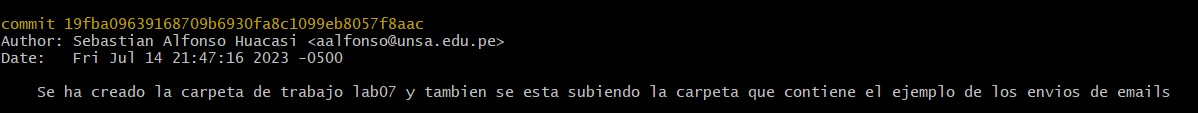
\includegraphics[width=0.8\textwidth,keepaspectratio]{img/1commit.jpg}
	%\includesvg{img/automata.svg}
	%\label{img:mot2}
	%\caption{Product backlog.}
\end{figure}
\begin{itemize}	
	\item Commit de la creacion de la carpeta de los ejemplos de model:
\end{itemize}
\begin{figure}[H]
	\centering
	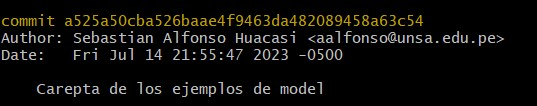
\includegraphics[width=0.8\textwidth,keepaspectratio]{img/2commit.jpg}
	%\includesvg{img/automata.svg}
	%\label{img:mot2}
	%\caption{Product backlog.}
\end{figure}
\begin{itemize}	
	\item Commit que indica que se estan subiendo la carpeta de los ejemplos de pdf y además los template:
\end{itemize}
\begin{figure}[H]
	\centering
	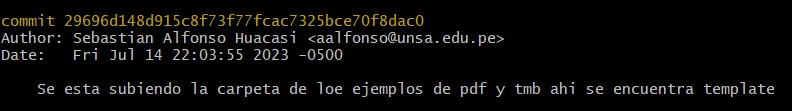
\includegraphics[width=0.8\textwidth,keepaspectratio]{img/3commit.jpg}
	%\includesvg{img/automata.svg}
	%\label{img:mot2}
	%\caption{Product backlog.}
\end{figure}
\begin{itemize}	
	\item Todo esto serían los archivos y orden de nuestro laboratorio 07:
\end{itemize}	
\begin{figure}[H]
	\centering
	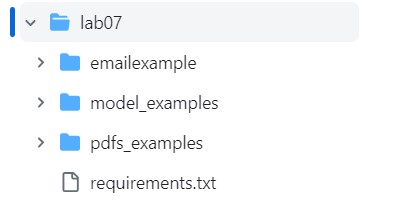
\includegraphics[width=0.8\textwidth,keepaspectratio]{img/estructura7.jpg}
	%\includesvg{img/automata.svg}
	%\label{img:mot2}
	%\caption{Product backlog.}
\end{figure}
\lstinputlisting[language=Python, caption={views.py-emails, se encuentra en la carpeta emailexample, dentro de la carpeta de send},numbers=left,]{src/views.py}
\begin{itemize}
        \item A continuación, procederé a explicar un poco el views.py de la parte de los emailsexample:
        \item from django.shortcuts import render: Importa la función render del módulo shortcuts de Django, que se utiliza para renderizar una plantilla y devolver una respuesta HTTP.
        \item from django.core.mail import send_mail: Importa la función send_mail del módulo mail de Django, que se utiliza para enviar correos electrónicos.
        \item def index(request): Define una función de vista llamada index que toma un objeto request como argumento. En Django, las funciones de vista se encargan de procesar las solicitudes HTTP y devolver respuestas.
        \item send_mail('Hola desde otra cuenta', 'Hello there. Esto es un mensaje automático.', 'sebastianalfonso2004@gmail.com', ['aalfonso@unsa.edu.pe'], fail_silently=False): Llama a la función send_mail para enviar un correo electrónico. Los parámetros proporcionados son:
        \item 'Hola desde otra cuenta': El asunto del correo electrónico.
        \item 'Hello there. Esto es un mensaje automático.': El cuerpo del correo electrónico.
        \item 'sebastianalfonso2004@gmail.com': La dirección de correo electrónico del remitente.
        \item ['aalfonso@unsa.edu.pe']: Una lista de direcciones de correo electrónico de los destinatarios.
        \item fail_silently=False: Indica que se debe generar una excepción si ocurre un error al enviar el correo electrónico.
        \item return render(request, 'send/index.html'): Renderiza la plantilla 'send/index.html' y devuelve la respuesta HTTP resultante. En este caso, la función de vista simplemente devuelve la plantilla sin modificar.
\end{itemize}
\lstinputlisting[language=Python, caption={views.py-pdfs, se encuentra en la carpeta pdfs_examples, dentro de la carpeta pdfs_example},numbers=left,]{src/viewss.py}
\begin{itemize}
        \item A continuación, procederé a explicar un poco el views.py de la parte de los pdfs_example:
        \item from django.http import HttpResponse: Importa la clase HttpResponse del módulo http de Django. HttpResponse se utiliza para devolver una respuesta HTTP desde una vista.
        \item from django.views.generic import View: Importa la clase View del módulo generic de Django. View es una clase base para vistas genéricas en Django.
        \item from django.template.loader import get_template: Importa la función get_template del módulo loader de Django. get_template se utiliza para cargar plantillas HTML.
        \item from .utils import render_to_pdf: Importa una función llamada render_to_pdf del módulo utils en el mismo directorio. Esta función se utiliza para generar un archivo PDF a partir de una plantilla HTML.
        \item def get(self, request, *args, **kwargs): Define un método get que manejará las solicitudes HTTP GET. Toma request y otros argumentos opcionales.
        \item template = get_template('pdf/invoice.html'): Carga la plantilla 'pdf/invoice.html' utilizando la función get_template.
        \item context = { ... }: Crea un diccionario context que contiene variables de contexto utilizadas en la plantilla. En este caso, incluye el número de factura, el nombre del cliente, el monto y la fecha actual.
        \item html = template.render(context): Renderea la plantilla con el contexto proporcionado, generando una cadena HTML.
        \item pdf = render_to_pdf('pdf/invoice.html', context): Genera un archivo PDF utilizando la función render_to_pdf y la plantilla junto con el contexto.
        \item response = HttpResponse(pdf, content_type='application/pdf'): Crea una instancia de HttpResponse con el contenido del archivo PDF y el tipo de contenido establecido como 'application/pdf'.
\end{itemize}
\subsection{Capturas de la ejecucion del laboratorio 07}
\begin{itemize}	
	\item Index email:
\end{itemize}	
\begin{figure}[H]
	\centering
	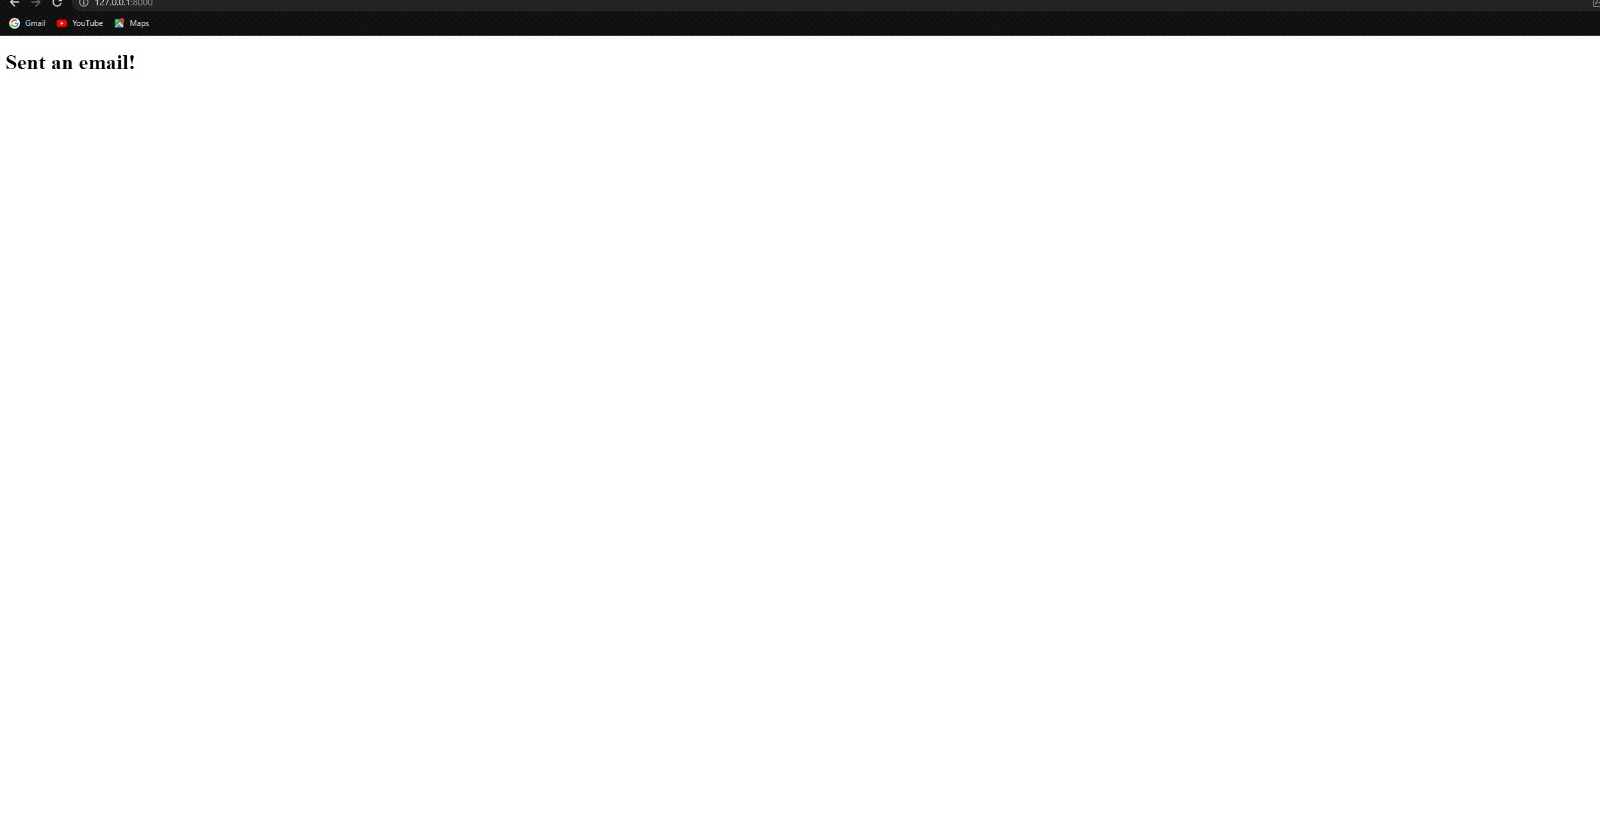
\includegraphics[width=0.8\textwidth,keepaspectratio]{img/index.jpeg}
	%\includesvg{img/automata.svg}
	%\label{img:mot2}
	%\caption{Product backlog.}
\end{figure}
\begin{itemize}	
	\item Demostración del pdf:
\end{itemize}	
\begin{figure}[H]
	\centering
	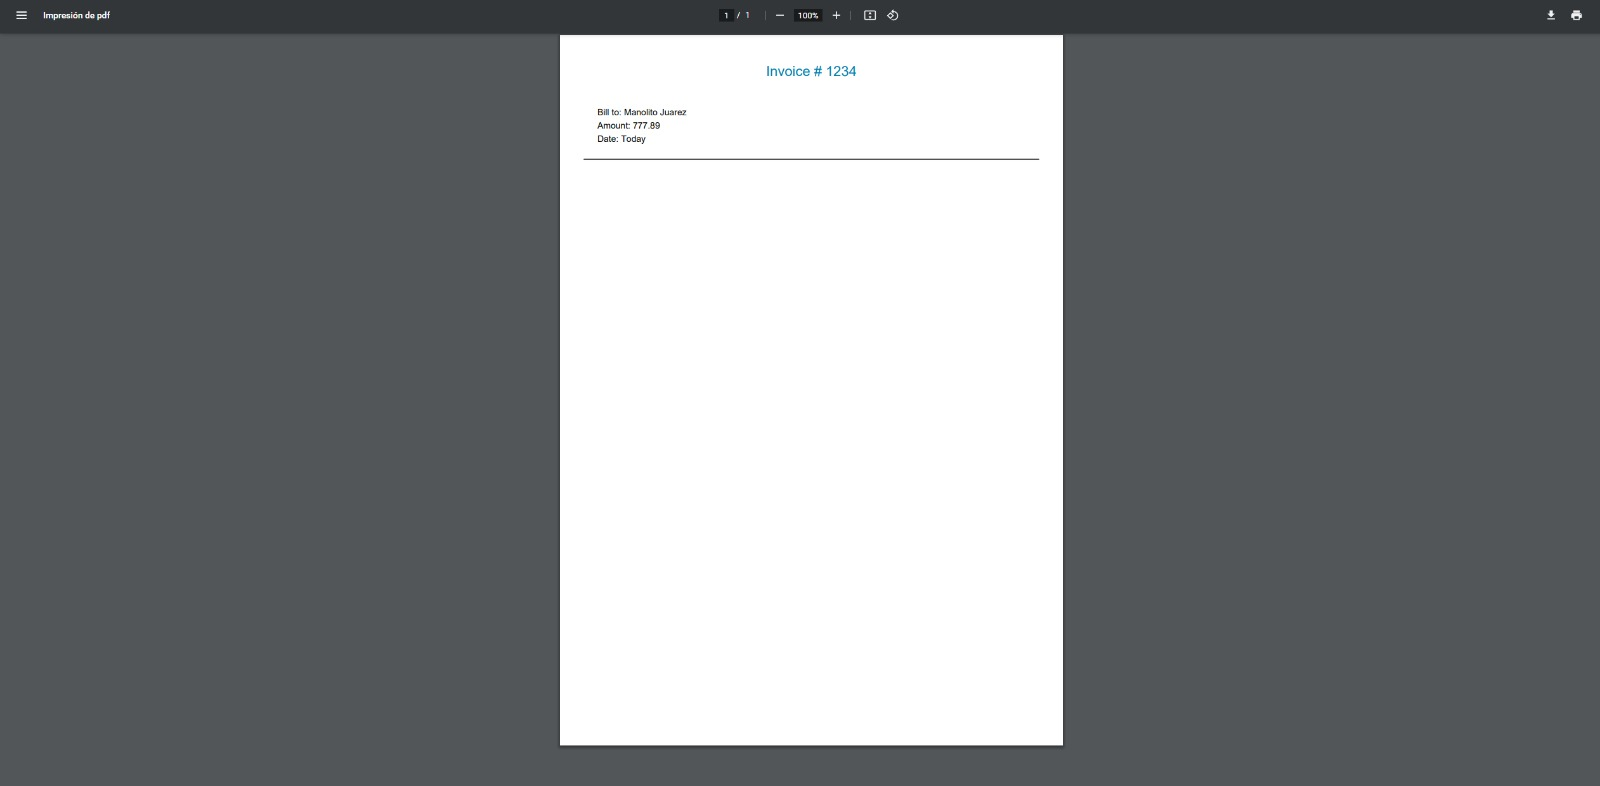
\includegraphics[width=0.8\textwidth,keepaspectratio]{img/pdf.jpeg}
	%\includesvg{img/automata.svg}
	%\label{img:mot2}
	%\caption{Product backlog.}
\end{figure}
\begin{itemize}	
	\item Email recibido, aumentandole algunas cosas más:
\end{itemize}	
\begin{figure}[H]
	\centering
	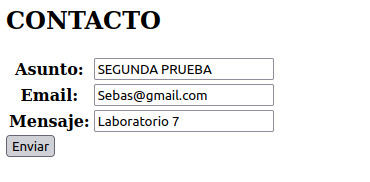
\includegraphics[width=0.8\textwidth,keepaspectratio]{img/e3.jpeg}
	%\includesvg{img/automata.svg}
	%\label{img:mot2}
	%\caption{Product backlog.}
\end{figure}
\begin{figure}[H]
	\centering
	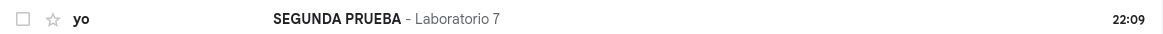
\includegraphics[width=0.8\textwidth,keepaspectratio]{img/e2.jpeg}
	%\includesvg{img/automata.svg}
	%\label{img:mot2}
	%\caption{Product backlog.}
\end{figure}
\begin{figure}[H]
	\centering
	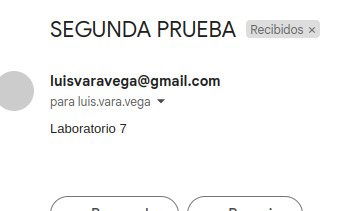
\includegraphics[width=0.8\textwidth,keepaspectratio]{img/e1.jpeg}
	%\includesvg{img/automata.svg}
	%\label{img:mot2}
	%\caption{Product backlog.}
\end{figure}
\begin{figure}[H]
	\centering
	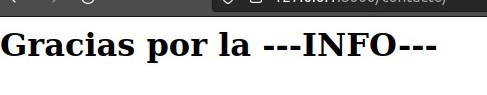
\includegraphics[width=0.8\textwidth,keepaspectratio]{img/e4.jpeg}
	%\includesvg{img/automata.svg}
	%\label{img:mot2}
	%\caption{Product backlog.}
\end{figure}
\subsection{Estructura de laboratorio 07}
\begin{itemize}	
	\item El contenido que se entrega del informe del laboratorio 07 es el siguiente:
\end{itemize}

\begin{lstlisting}[style=ascii-tree]
	Lab07-Informe/
   |--- informe-latex
	|--- contenido
   |   |--- actividades.tex
   |   |--- caratula.tex
   |   |--- github.tex
   |   |--- materiales.tex
   |   |--- preguntas.tex
   |   |--- referencia.tex
   |   |--- rubrica.tex
   |   |--- tarea.tex
	|--- img
   |   |--- logo_abet.png
   |   |--- logo_episunsa.png
   |   |--- logo_unsa.jpg
   |   |--- 1commit.jpg
   |   |--- 2commit.jpg
   |   |--- 3commit.jpg
   |   |--- e1.jpeg
   |   |--- e2.jpeg
   |   |--- e3.jpeg
   |   |--- e4.jpeg
   |   |--- estructura7.jpg
   |   |--- index.jpeg
   |   |--- pdf.jpeg
   |--- src
   |    |--- views.py
   |    |--- viewss.py
   |--- pweb2_lab07_aalfonso.pdf    
   |--- main.tex
\end{lstlisting}    

	\section{Pregunta: Como te fue con el trabajo del laboratorio 07?}
\begin{itemize}
	\item Fue un laboratorio interesante para realizarlo con algunas dificultades, pero se pudo terminar. Realizando los 4 puntos que se pedía.
\end{itemize}


	\section{\textcolor{red}{Rúbricas}}

\subsection{\textcolor{red}{Entregable Informe}}
\begin{table}[H]
	\caption{Tipo de Informe}
	\setlength{\tabcolsep}{0.5em} % for the horizontal padding
	{\renewcommand{\arraystretch}{1.5}% for the vertical padding
		\begin{tabular}{|p{3cm}|p{12cm}|}
			\hline
			\multicolumn{2}{|c|}{\textbf{\textcolor{red}{Informe}}}  \\
			\hline 
			\textbf{\textcolor{red}{Latex}} & \textcolor{blue}{El informe está en formato PDF desde Latex,  con un formato limpio (buena presentación) y facil de leer.}   \\ 
			\hline 
			
			
		\end{tabular}
	}
\end{table}

\subsection{\textcolor{red}{Rúbrica para el contenido del Informe y demostración}}
\begin{itemize}			
	\item El alumno debe marcar o dejar en blanco en celdas de la columna \textbf{Checklist} si cumplio con el ítem correspondiente.
	\item Si un alumno supera la fecha de entrega,  su calificación será sobre la nota mínima aprobada, siempre y cuando cumpla con todos lo items.
	\item El alumno debe autocalificarse en la columna \textbf{Estudiante} de acuerdo a la siguiente tabla:
	
	\begin{table}[ht]
		\caption{Niveles de desempeño}
		\begin{center}
			\begin{tabular}{ccccc}
				\hline
				& \multicolumn{4}{c}{Nivel}\\
				\cline{1-5}
				\textbf{Puntos} & Insatisfactorio 25\%& En Proceso 50\% & Satisfactorio 75\% & Sobresaliente 100\%\\
				\textbf{2.0}&0.5&1.0&1.5&2.0\\
				\textbf{4.0}&1.0&2.0&3.0&4.0\\
				\hline
			\end{tabular}
		\end{center}
	\end{table}	
	
\end{itemize}

\begin{table}[H]
	\caption{Rúbrica para contenido del Informe y demostración}
	\setlength{\tabcolsep}{0.5em} % for the horizontal padding
	{\renewcommand{\arraystretch}{1.5}% for the vertical padding
		%\begin{center}
		\begin{tabular}{|p{2.7cm}|p{7cm}|x{1.3cm}|p{1.2cm}|p{1.5cm}|p{1.1cm}|}
			\hline
			\multicolumn{2}{|c|}{Contenido y demostración} & Puntos & Checklist & Estudiante & Profesor\\
			\hline
			\textbf{1. GitHub} & Hay enlace URL activo del directorio para el  laboratorio hacia su repositorio GitHub con código fuente terminado y fácil de revisar. &2 &X &2 & \\ 
			\hline
			\textbf{2. Commits} &  Hay capturas de pantalla de los commits más importantes con sus explicaciones detalladas. (El profesor puede preguntar para refrendar calificación). &4 &X &2 & \\ 
			\hline 
			\textbf{3. Código fuente} &  Hay porciones de código fuente importantes con numeración y explicaciones detalladas de sus funciones. &2 &X &1 & \\ 
			\hline 
			\textbf{4. Ejecución} & Se incluyen ejecuciones/pruebas del código fuente  explicadas gradualmente. &2 &X &2 & \\ 
			\hline			
			\textbf{5. Pregunta} & Se responde con completitud a la pregunta formulada en la tarea.  (El profesor puede preguntar para refrendar calificación).  &2 &X &2 & \\ 
			\hline	
			\textbf{6. Fechas} & Las fechas de modificación del código fuente estan dentro de los plazos de fecha de entrega establecidos. &2 &X &2 & \\ 
			\hline 
			\textbf{7. Ortografía} & El documento no muestra errores ortográficos. &2 &X &2 & \\ 
			\hline 
			\textbf{8. Madurez} & El Informe muestra de manera general una evolución de la madurez del código fuente,  explicaciones puntuales pero precisas y un acabado impecable.   (El profesor puede preguntar para refrendar calificación).  &4 &X &3 & \\ 
			\hline
			\multicolumn{2}{|c|}{\textbf{Total}} &20 & &16 & \\ 
			\hline
		\end{tabular}
		%\end{center}
		%\label{tab:multicol}
	}
\end{table}

\clearpage
	
	\section{Referencias}
\begin{itemize}			
	\item \url{https://www.w3schools.com/python/python_reference.asp}
        \item \url{https://docs.djangoproject.com/en/4.2/howto/outputting-pdf/}
        \item\url{https://www.scaler.com/topics/django/relationships-in-django-models/}
        \item\url{https://docs.djangoproject.com/en/4.2/topics/email/}
\end{itemize}	
			
\end{document}